\documentclass{article}
\usepackage[margin=1in]{geometry}
\usepackage{graphics}
\usepackage{common}
\usepackage{pagesetup}
\usepackage{placeins}
\usepackage{tikz}
\usetikzlibrary{calc, arrows.meta, positioning}

\newcommand{\N}{\mathcal{N}}

\begin{document}

\lecture{8}{September 27}{Sasha Rush}{Giridhar Anand, Michael Xueyuan Han, Ana-Roxana Pop}{Backpropagation \& Directed Graphical Models}

\subsection{Backpropagation in Neural Networks}
\subsubsection{Neural networks review}
\noindent
In the last lecture, we defined the mean parameter of a neural network as follows:
\[\mu = \sigma(w^T\text{ReLU}(Wx))\]
Here, $\mu$ parameterizes a Bernoulli distribution, $\text{Ber}(\mu)$. Suppose we want to find $\mu$ such that it maximizes the likelihood of a single data example $(x, y)$. Then we compute \[ \mu = \argmax{\mu}\log{p(y|x)} = \argmin_\mu \left(-\log{p(y\given x)}\right) = \argmin_\mu L\]
where $L$ is the loss of the neural network.
\subsubsection{Chain rule and backpropagation}
We can represent the neural network graphically as follows:\\
\begin{center}
\begin{tikzpicture}[
  node/.style={ellipse,draw=black},
  edge/.style={-Stealth},
  node distance=0.5in and 1in
  ]
  \node[node] (c1){$x_2$};
  \node[node, above=of c1](c2){$x_1$};
  \node[node, below=of c1](c3){$x_3$};
  \node[node, right=of c1](c4){$\text{ReLU(Wx)}_3$};
  \node[node, above=of c4](c5){$\text{ReLU(Wx)}_2$};
  \node[node, below=of c4](c6){$\text{ReLU(Wx)}_4$};
  \node[node, above=of c5](c7){$\text{ReLU(Wx)}_1$};
  \node[node, below=of c6](c8){$\text{ReLU(Wx)}_5$};
  \node[node, right=of c4](c9){$L$};

\foreach \i/\j in {% start node/end node
  c1/c4, c1/c5, c1/c6, c1/c7, c1/c8,
  c2/c4, c2/c5, c2/c6, c2/c7, c2/c8,
  c3/c4, c3/c5, c3/c6, c3/c7, c3/c8,
  c4/c9, c5/c9, c6/c9, c7/c9, c8/c9}
  \draw [edge] (\i) -- (\j);
\end{tikzpicture}
\end{center}

\noindent
In order to generate this graph, we must perform the following computational operations in order:
\[
\begin{array}{*{11}c}
v^{(0)} & \rightarrow & v^{(1)} & \rightarrow & v^{(2)} & \rightarrow & v^{(3)} & \rightarrow & v^{(4)} & \rightarrow & L\\
x && Wv^{(0)} && \text{ReLU}(v^{(1)}) && w^Tv^{(2)} && \sigma(v^{(3)}) && -\log{v^{(4)}}\\
\end{array}
\]
We would like to get the gradient terms $\dot{v}^{(i)} \equiv \frac{d L}{d v^{(i)}}$ for any $i$, which tell us how each part of the neural network affects our loss. We can do this by applying the chain rule (of calculus) to get a recursive solution (by convention, the derivative of a scalar with respect to a vector is represented as a column vector):
\[
\frac{d L}{d v^{(i)}} = \left( \frac{d L}{d v^{(i+1)}}\right)^T \frac{d v^{(i+1)}}{d v^{(i)}}
\]

\[
\frac{\partial L}{\partial v_k^{(i)}} = \sum_j \frac{\partial L}{\partial v_j^{(i+1)}} \frac{\partial v_j^{(i+1)}}{\partial v^(i)}
\]

\noindent
Since the gradient of each term depends on the gradient of the subsequent term, we can compute the gradients in reverse while applying the chain rule. This method is known as backpropagation. For each backward step, we need to remember everything that was computed in the corresponding forward step, namely $v^{(i)}$, $\dot{v}^{(i+1)}$, and $\frac{d v^{(i+1)}}{d v^{(i)}}$:

\[
\begin{array}{*{11}c}
v^{(0)} & \rightarrow & v^{(1)} & \rightarrow & v^{(2)} & \rightarrow & v^{(3)} & \rightarrow & v^{(4)} & \rightarrow & L\\
\vspace{.35cm}
x && Wv^{(0)} && \text{ReLU}(v^{(1)}) && w^Tv^{(2)} && \sigma(v^{(3)}) && -\log{v^{(4)}}\\
\dot{v}^{(0)} & \leftarrow & \dot{v}^{(1)} & \leftarrow & \dot{v}^{(2)} & \leftarrow & \dot{v}^{(3)} & \leftarrow & \dot{v}^{(4)} & \leftarrow &\\
...&&...&& (\dot{v}^{(2)})^T W &&\dot{\sigma}(v^{(3)})\dot{v}^{(4)}&&-\frac{1}{v^{(4)}}&&
\end{array}
\]

\subsubsection{Writing software for neural networks}
\begin{itemize}
\item ``blocks'' style neural network (e.g. Torch)

Computation is done in ``blocks'' which are black boxes $f$  that implement the following contract:

\tikzstyle{block} = [draw, rectangle, minimum size=1.5in]
\begin{tikzpicture}[>=stealth,auto, node distance=1in]
    \node [block] (model) {$\displaystyle \frac{d v^{(i+1)}}{d v^{(i)}}$};
    \draw [<-] ($(model.north west)!0.5!(model.west)$) -- node {input, $v^{(i)}$} +(-1in,0pt);
    \draw [->] ($(model.west)!0.5!(model.south west)$) -- node {grad input, $\dot{v}^{(i)}$}+(-1in,0pt);
    \draw[->] ($(model.north east)!0.5!(model.east)$) -- node {output, $v^{(i+1)}$}+(1.25in,0pt);
	\draw[<-] ($(model.east)!0.5!(model.south east)$) -- node {grad output, $\dot{v}^{(i+1)}$} +(1.25in,0pt);
\end{tikzpicture}

We can also augment the black boxes. For instance, if we let $f$ take in parameter $W$, we can also compute $\frac{d L}{d W}$ within this function.

\item computational graph (e.g. Theano, TensorFlow)

Everything is implemented in terms of primitives, so there are no black boxes:

\tikzstyle{block} = [draw, rectangle, minimum size=1.5in]
\begin{tikzpicture}[>=stealth,auto, node distance=1in]
    \node [block] (model) {$\displaystyle +, \times, ...$};
    \draw [<-] ($(model.north west)!0.5!(model.west)$) -- node {} +(-1in,0pt);
    \draw [->] ($(model.west)!0.5!(model.south west)$) -- node {}+(-1in,0pt);
    \draw[->] ($(model.north east)!0.5!(model.east)$) -- node {}+(1.25in,0pt);
	\draw[<-] ($(model.east)!0.5!(model.south east)$) -- node {} +(1.25in,0pt);
\end{tikzpicture}

This allows us to optimize the neural network once and run it on many examples.

\item imperative/autograd systems

These are tape-based systems in which the computational graph can look different for different examples, but we can still compute gradients using backpropagation. Torch is built on an autograd core, but higher level functions like the Linear module take on a ``blocks'' style approach.

\end{itemize}

\subsection{Graphical Models}
\subsubsection{Directed Graphical Models}

The goal of using directed graphical models (DGMs) is to separate out two parts of a model:
\begin{enumerate}
\item Conditional Independence
\item Parameters and Parametrization
\end{enumerate}

\begin{figure}[!ht]
    \centering
    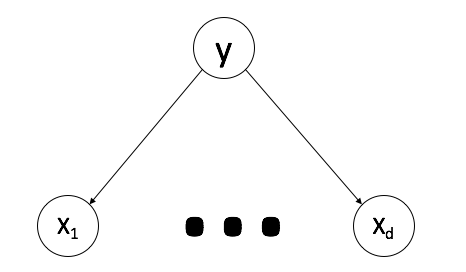
\includegraphics[width = 0.4\textwidth]{nb1.png}
    %\vspace{-0.2cm}
    \caption{The graphical model of Naive Bayes}
    %\vspace{-0.5cm}
    \label{fig:nb1}
\end{figure}


\noindent
In the case of Naive Bayes (see Figure \ref{fig:nb1}), we know from a previous lecture that:
\begin{itemize}
\item $p(y)$ is probably categorical.
\item $p(x_{j}|y)$ could be one of many different distributions, including Categorical, Gaussian, Bernoulli, etc.
\end{itemize}
We are interested in the following distributions from the underlying data that we have:
\begin{itemize}
\item p(y, x): joint distribution
\item $p(x_{j})$: marginal distribution, or $p(y \mid x)$: conditional distribution
\end{itemize}



\emph{The structure of the model will often determine the difficulty of inference}. This is the motivation of why we want to draw these graphs.



On a high level,
given $p(A, B, C)$, we can always apply the chain rule (in probability):
\[ 
p(A, B, C) = p(A \mid B, C) \, p(B \mid C) \, p(C) 
\]
However, if we write $p(A, B, C)$ in the way above, we basically assume that all variables depend on each other. In some cases, this is not necessarily true, and we want to find a factorization as below. 

\subsubsection{Factorization}
If we have the case presented in Figure \ref{fig:nb2}, we can rewrite $p(A \mid B, C) \rightarrow p(A \mid B)$.
Having A only depend on one variable (B) is better than having it depend on two variables (B and C).
\begin{figure}[!ht]
    \centering
    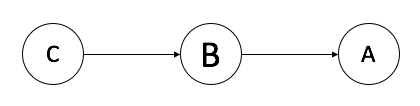
\includegraphics[width = 0.4\textwidth]{nb2.png}
    %\vspace{-0.2cm}
    \caption{A graph where factorization is possible.}
    %\vspace{-0.5cm}
    \label{fig:nb2}
\end{figure}


\subsubsection{Formalism of DGMs}
\noindent
Formally, for directed graphical models (DGMs) (or \emph{Bayes Nets}, or \emph{causal graphs}) we have:
\begin{itemize}
\item A graph $G=(V, E)$ where $(s, t) \in E, s \neq t$ (V are vertices, E are edges)
\item Each node is a random variable.
\item Each edge is a conditioning decision.
\item The graph is topologically ordered and it is a directed acyclic graph (DAG).
\item Notation: $\mathrm{pa}(x)$ represents $x$'s parents.
\end{itemize}

\subsubsection{Parents notation}
Here, $A$ and $B$ are independent of each other, and they are $C$'s parents (as in Figure \ref{fig:nb3}). We can then write:
\begin{figure}[!ht]
    \centering
    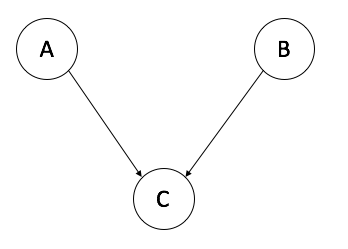
\includegraphics[width = 0.35\textwidth]{nb3.png}
    %\vspace{-0.2cm}
    \caption{A graph to illustrate the use of parents notation.}
    %\vspace{-0.5cm}
    \label{fig:nb3}
\end{figure}
\[
p(A, B, C) = p(A)\, p(B)\, p(C \mid A, B) = p(A) \, p(B) \, p(C \mid \mathrm{pa}(C))
\]



\FloatBarrier
\subsubsection{Plate Notation}
When we have lots of exchangeable variables (i.e., order is not important), we can use the \emph{plate} notation.
We want to graphically represent Naive Bayes on examples $(x_j^{(n)}, y^{(n)})$, in which
\begin{itemize}
\item $y$ is parameterized on $\pi$: $p(y^{(n)} \mid \pi)$, and
\item $x_{j}$ depends on $y$ and $\mu$: $p(x_{j}^{(n)} \mid y, \mu)$
\end{itemize}
Since we have $n$ samples of $(x, y)$, we can use the plate notation, as shown in Figure \ref{fig:nb4}.
\begin{figure}[!ht]
    \centering
    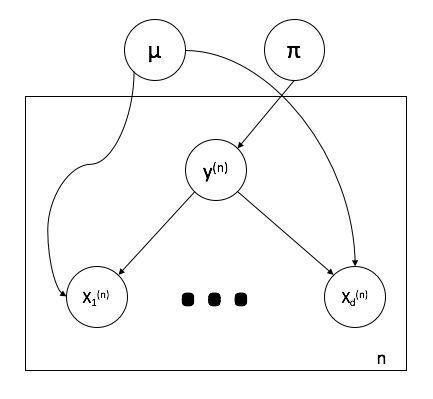
\includegraphics[width = 0.5\textwidth]{nb4.png}
    %\vspace{-0.2cm}
    \caption{A graph to illustrate the use of plate notation.}
    \label{fig:nb4}
    %\vspace{-0.5cm}
\end{figure}
\FloatBarrier


\subsubsection{Caching probabilities}
You can save ``probabilities'' in the model, which is simply \emph{caching} the values of probabilities with the graph. 
In this case (Figure \ref{fig:nb5}), variables are discrete. We call $C$'s probability table \emph{conditional probability table (CPT)} since it is conditioned on $A, B$. Note that the values do not tell us anything about how the distribution is parameterized. Those are simply the probability values that you can read off from the graph.

Note also that the CPT of $p(x_{i} \mid x_{1}, \cdots, x_{i - 1})$ = $O(\prod_{i} |x_{i} |)$ (i.e., exponential growth with the number of conditional terms). 
\begin{figure}[!ht]
    \centering
    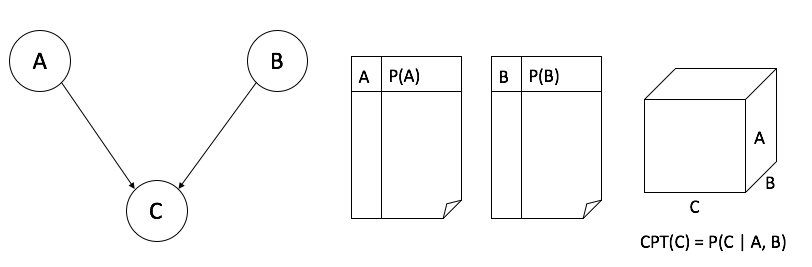
\includegraphics[width = 0.6\textwidth]{nb5.png}
    %\vspace{-0.2cm}
    \caption{A model with probability tables. The CPT of C is a three-dimensional table.}
    %\vspace{-0.5cm}
    \label{fig:nb5}
\end{figure}



\FloatBarrier
\subsubsection{Examples of Directed Graphical Models}
\begin{example}[Markov Chain]
Figure \ref{fig:nb6} shows an example of a Markov chain graphical model.
\begin{figure}[!ht]
    \centering
    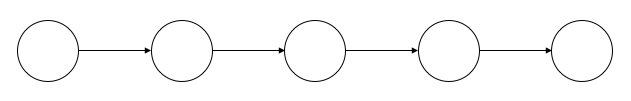
\includegraphics[width = 0.4\textwidth]{nb6.png}
    %\vspace{-0.2cm}
    \caption{Markov Chain Graphical Model}
    \label{fig:nb6}
    %\vspace{-0.5cm}
\end{figure}
\end{example}

\begin{example}[Second Order Markov Chain]
Figure \ref{fig:nb7} shows an example of a second order Markov chain graphical model.
\begin{figure}[!ht]
    \centering
    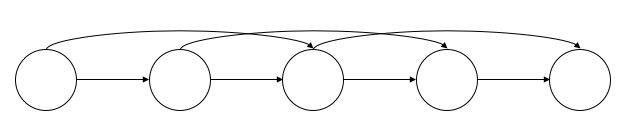
\includegraphics[width = 0.4\textwidth]{nb7.png}
    %\vspace{-0.2cm}
    \caption{Second Order Markov Chain Graphical Model}
    \label{fig:nb7}
    %\vspace{-0.5cm}
\end{figure}
\end{example}

\begin{example}[Hidden Markov Model]
Figure \ref{fig:nb8} shows an example of a hidden Markov graphical model.
\begin{figure}[!ht]
    \centering
    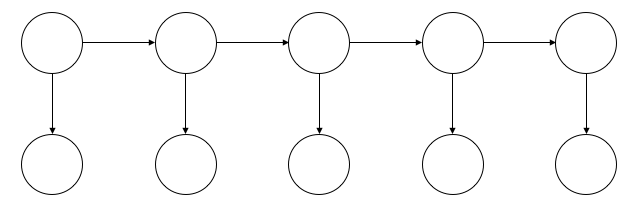
\includegraphics[width = 0.4\textwidth]{nb8.png}
    %\vspace{-0.2cm}
    \caption{Hidden Markov Graphical Model}
    %\vspace{-0.5cm}
    \label{fig:nb8}
\end{figure}
\end{example}

\begin{example}[Navie Bayes]
Figure \ref{fig:nb9} shows an example of a Naive Bayes graphical model.
\begin{figure}[!ht]
    \centering
    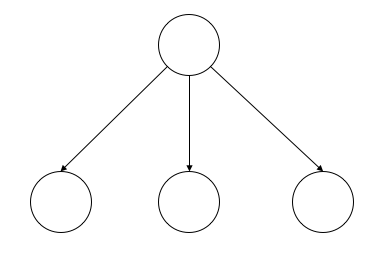
\includegraphics[width = 0.25\textwidth]{nb9.png}
    %\vspace{-0.2cm}
    \caption{Naive Bayes Graphical Model}
    %\vspace{-0.5cm}
    \label{fig:nb9}
\end{figure}
\end{example}
\FloatBarrier

As we have seen in Figure \ref{fig:nb4}, we can also incorporate parameters in the DGMs, as it is illustrated in the next example.
\begin{example}
In this case (Figure \ref{fig:nb10}), we use the same Naive Bayes example with parameters. Here, we incorporate parameters $\alpha \sim \on{Dirichlet}$. This is interesting because it combines two types of distributions: some of them are discrete, but in this example $\alpha$ and $\pi$ are drawn from continuous distributions, as marked in the figure below.
\begin{figure}[!ht]
    \centering
    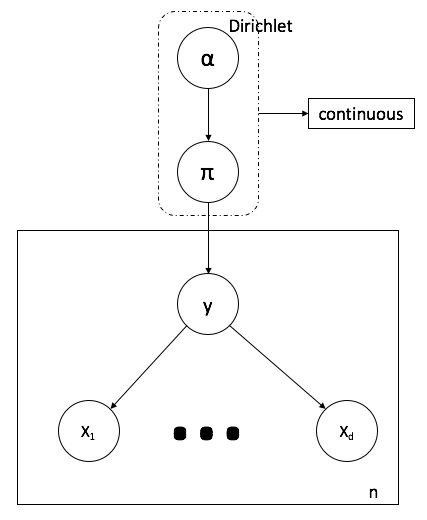
\includegraphics[width = 0.5\textwidth]{nb10.png}
    %\vspace{-0.2cm}
    \caption{Naive Bayes Graphical Model with Parameters}
    %\vspace{-0.5cm}
    \label{fig:nb10}
\end{figure}
\end{example}
\FloatBarrier
Figure \ref{fig:nb10} corresponds to a single example. 
If we have multiple examples, we can use a plate-in-plate representation as in Figure \ref{fig:nb11}. 
\begin{figure}[!ht]
    \centering
    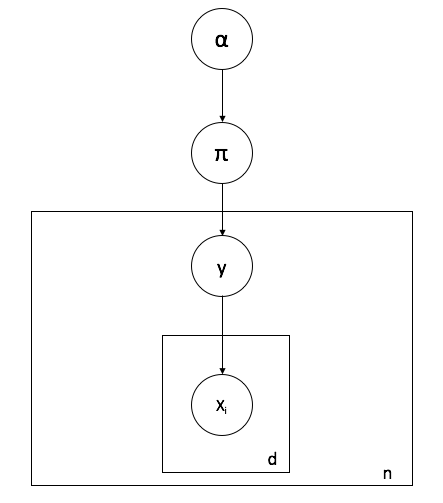
\includegraphics[width = 0.5\textwidth]{nb11.png}
    %\vspace{-0.2cm}
    \caption{Naive Bayes Graphical Model with Parameters and Plate-in-Plate Notation}
    %\vspace{-0.5cm}
    \label{fig:nb11}
\end{figure}

\subsection{Gaussian Directed Models}
Gaussian directed models are a special case of DGMs where every one of the variables has the following distribution:
\[
p(x_i \mid \mathrm{pa}(x_i)) = \N (x_i \mid \mu_i + \sum_{j = \mathrm{pa}(x_i)} W_{ij} (x_{ij} - \mu_j), \;\; \sigma_i^2) 
\]
In the above equation, we transform each of the $\mu_i$ based on the starting mean plus a linear transformation of their parents (and to simplify things, we subtract the mean of each parent). We have an underlying generative process where each one of our random variables is a draw from a Gaussian and its children  are a linear transformations of that draw.

This means that, we can rewrite $x_{i}$ as:
\[
x_i = \mu_i + \sum_j W_{ij} (x_j - \mu_j) + \sigma_i z_i \;\;\;\;\; \forall i \;\; z_i \sim \N(0,1)
\]
Notice that $\sigma_i z_i$ is just Gaussian random noise.

If we define $S = \mathrm{diag} (\sigma)$ (where each term will contribute a different corresponding $\sigma_i$), we can rewrite the above equation in a matrix form:
\[
(x_i - \mu_i) = W(x-\mu) + S z
\]
where $\mu = \left[ \mu_1, \cdots, \mu_d\right]$ is a vector containing each individual means.

By rearranging the terms, we find:
\begin{align*}
S z &= (I - W) (x - \mu)\\
x - \mu &= (I-W)^{-1} S z 
\end{align*}
This tells us how the $x$ random variable differs from the mean at each of the different positions.

We know that the $\Sigma$ term for our covariant matrix is defined as:
\begin{align*} 
\Sigma \equiv \cov \left[x - \mu \right] &= \cov \left[ (I - W)^{-1} S \,z \right] \\
&= (I - W)^{-1} S \, \cov \left[ z \right] \, S ((I-W)^{-1})^T\\
&= (I - W)^{-1} \, S^2 \, ((I-W)^{-1})^T
\end{align*}
which means that, in general, for Gaussian DGMs we have:
\[
\text{Gaussian DGM} \sim \N(\mu,\, (I - W)^{-1} \, S^2 \,  ((I-W)^{-1})^T)
\]
\begin{remark}
We will talk about \emph{D-Separation} in the next lecture.
\end{remark}
\end{document}

